\documentclass{article}

\usepackage{graphicx}
\usepackage{tikz}
\usepackage{tikzsymbols}
\usetikzlibrary{calc,patterns,shapes.geometric}
\pagestyle{empty}
\usepackage[margin=0pt]{geometry}
\geometry{papersize={14in,12in}}

\def\centerarc[#1](#2)(#3:#4:#5){\draw[#1] ($(#2)+({#5*cos(#3)},{#5*sin(#3)})$) arc (#3:#4:#5);}

\begin{document}
	\begin{figure}
		\centering
		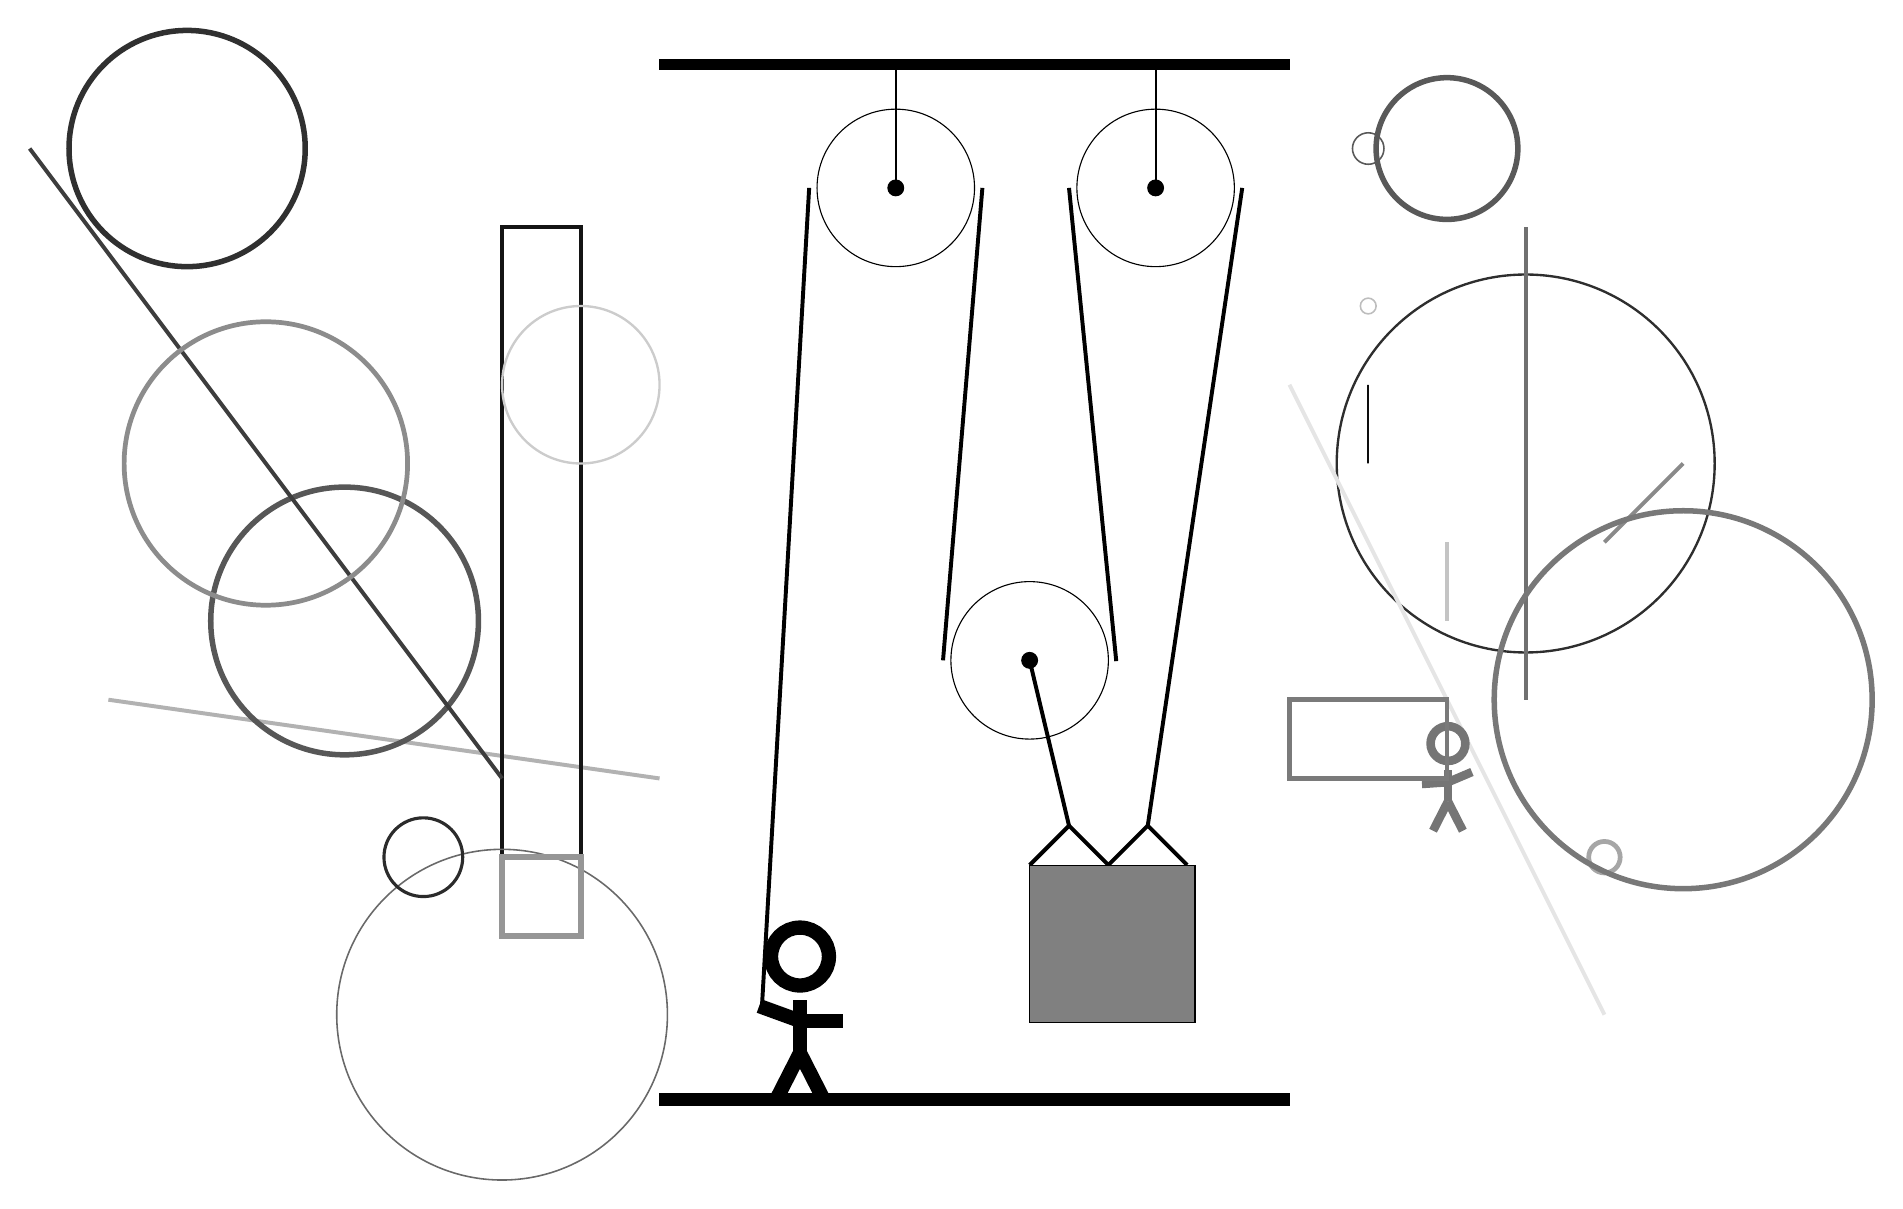
\begin{tikzpicture}
			%%%%% START %%%%%
			
			\draw[fill=black] (-2, 10) rectangle (6, 10.125);
			
			\draw (1, 8.5) circle (1);
			\draw[fill=black] (1, 8.5) circle (0.1);
			\draw[thick] (1, 8.5) -- (1, 10);
			
			\draw (4.3, 8.5) circle (1);
			\draw[fill=black] (4.3, 8.5) circle (0.1);
			\draw[thick] (4.3, 8.5) -- (4.3, 10);
			
			\draw (2.7, 2.5) circle (1);
			\draw[fill=black] (2.7, 2.5) circle (0.1);
			
			\draw[line width=0.5mm]  (2.7, -0.1) -- (3.2, 0.4) -- (3.7, -0.1) -- (4.2, 0.4) -- (4.7, -0.1);
			\draw[fill=black!50] (2.7, -0.1) rectangle (4.8, -2.1);
			
			\draw[line width=0.5mm](-0.7, -1.9) -- (-0.1, 8.5);
			\centerarc[line width=0.5mm](1, 8.5)(0:180:1.1);
			\draw[line width=0.5mm](2.1, 8.5) -- (1.6, 2.5);
			\centerarc[line width=0.5mm](2.7, 2.5)(180:370:1.1);
			\draw[line width=0.5mm] (3.8, 2.49) -- (3.2, 8.5);
			\centerarc[line width=0.5mm](4.3, 8.5)(0:180:1.1);
			\draw[line width=0.5mm](4.2, 0.4) -- (5.4, 8.5);
			\draw[line width=0.5mm] (3.2, 0.4) -- (2.7, 2.5);
			
			\draw [line width=0.3mm, color=black!82](9, 5) circle (2.4);
			
			\draw[line width=0.5mm, color=black!56](9, 8) -- (9, 2);
			\draw[line width=0.5mm, color=black!46](11, 5) -- (10, 4);
			\draw[line width=0.5mm, color=black!23] (8, 3) rectangle (8, 4);
			
			\draw[line width=0.5mm, color=black!30](-2, 1) -- (-9, 2);
			
			\draw [line width=0.7mm, color=black!66](-6, 3) circle (1.7);
			\draw[line width=0.5mm, color=black!92] (-4, 0) rectangle (-3, 8);
			\draw[line width=0.5mm, color=black!76](-4, 1) -- (-10, 9);
			\draw [line width=0.2mm, color=black!26](7, 7) circle (0.1);
			\draw [line width=0.3mm, color=black!20](-3, 6) circle (1.0);
			
			\draw[line width=0.5mm, color=black!10](10, -2) -- (6, 6);
			
			\draw [line width=0.6mm, color=black!35](10, 0) circle (0.2);
			\draw [line width=0.7mm, color=black!65](8, 9) circle (0.9);
			
			\draw[line width=0.3mm, color=black!95] (7, 6) rectangle (7, 5);
			\draw [line width=0.2mm, color=black!65](7, 9) circle (0.2);
			\draw [line width=0.7mm, color=black!53](11, 2) circle (2.4);
			
			\draw [line width=0.6mm, color=black!45](-7, 5) circle (1.8);
			
			\draw [line width=0.2mm, color=black!59](-4, -2) circle (2.1);
			\draw[line width=0.7mm, color=black!41] (-4, 0) rectangle (-3, -1);
			\node[line width=0.2mm, color=black!54] at (8, 1) {\Strichmaxerl[6][4][23]};
			\draw [line width=0.7mm, color=black!81](-8, 9) circle (1.5);
			\draw [line width=0.4mm, color=black!83](-5, 0) circle (0.5);
			\draw[line width=0.6mm, color=black!52] (6, 2) rectangle (8, 1);
			
			\node at (-0.2, -2) {\Strichmaxerl[10][-20][0]};
			
			\draw[fill=black] (-2, -3) rectangle (6, -3.15);
			
			%%%%% END %%%%%
		\end{tikzpicture}
	\end{figure}	
\end{document}